\section{线性化与切空间}\label{sec:linearizations-and-tangent-spaces}

切线和切平面在大多数一元和多元微积分课程中都占有重要地位. 这些课程通常先用极限定义导数, 再利用极限定义推出标准的求导法则. 例如, 一条标准的求导法则说, 对任意 $k\in\mathbb{N}$, $x^{k}$ 的导数为 $kx^{k-1}$. 由于极限在一般基域 $K$ 上没有意义, 我们在代数几何中讨论相切时, 不从极限出发, 而从多项式的求导法则出发.

我们假设读者熟悉多元多项式的标准求导法则, 并把这些公式推广到任意环 $R$. 换句话说, 若
\[
  f=a_{m}x^{m}+a_{m-1}x^{m-1}+\cdots+a_{1}x+a_{0}\in R[x],
\]
则 $f$ 关于 $x$ 的导数定义为
\[
  \frac{\partial f}{\partial x}=ma_{m}x^{m-1}+(m-1)a_{m-1}x^{m-2}+\cdots+a_{1}\in R[x],
\]
其中 $ma_{m}$ 表示 $m$ 个 $a_{m}$ 相加. 若 $f\in R[x_{1},\ldots,x_{n}]$ 是多元多项式, 那么对于每个变量 $x_{i}$, 可把 $f$ 看作 $R'[x_{i}]$ 的元素来求导, 从而定义偏导数 $\partial f/\partial x_{i}$. 这里
\[
  R'=R[x_{1},\ldots,x_{i-1},x_{i+1},\ldots,x_{n}].
\]
利用这些偏导数, 给出建立切空间所需的关键定义.

\begin{Definition}{多项式在一点处的线性化}\leavevmode\label{def:linearization-of-polynomial}
若 $f\in K[x_{1},\ldots,x_{n}]$, 且 $a=(a_{1},\ldots,a_{n})\in\mathbb{A}^{n}$, 则 $f$ 在 $a$ 处的\emph{线性化}定义为
\[
  L_{a}f=f(a)+\sum_{i=1}^{n}\left(\frac{\partial f}{\partial x_{i}}(a)\right)\cdot(x_{i}-a_{i})
    \in K[x_{1},\ldots,x_{n}].
\]
\end{Definition}

注意 $\frac{\partial f}{\partial x_{i}}\in K[x_{1},\ldots,x_{n}]$ 是一个多项式, 而 $\frac{\partial f}{\partial x_{i}}(a)\in K$ 表示该多项式在 $a$ 处的值, 所以 $L_{a}f\in K[x_{1},\ldots,x_{n}]$ 是线性多项式. 在多元微积分中 (换句话说, 当 $K=\mathbb{R}$ 时), $f$ 在 $a$ 处的线性化被引入为在 $a$ 附近最接近 $f$ 的线性函数. 它有时也称为 $f$ 在 $a$ 处的\emph{线性近似}.

仿射簇在一点处的线性化定义为其消没理想中所有多项式的线性化的共同零点集.

\begin{Definition}{仿射簇在一点处的线性化}\leavevmode\label{def:linearization-of-affine-variety}
设 $X\subseteq\mathbb{A}^{n}$ 是仿射簇, 且 $a\in X$. $X$ 在 $a$ 处的\emph{线性化}是
\[
  L_{a}X=\mathcal{V}\bigl(\{L_{a}f\mid f\in\mathcal{I}(X)\}\bigr)\subseteq\mathbb{A}^{n}.
\]
\end{Definition}

建议读者验证 (Exercise~\ref{ex:linearization-and-tangency-from-generators}), 若 $\mathcal{I}(X)=\langle f_{1},\ldots,f_{m}\rangle$, 则
\[
  L_{a}X=\mathcal{V}(L_{a}f_{1},\ldots,L_{a}f_{m}).
\]
由于每个消没理想都是有限生成的, 这意味着总可用一组有限个线性多项式定义线性化. 还要注意, 每个 $L_{a}f_{i}$ 定义中的第一项 $f_{i}(a)$ 都为零, 因为 $f_{i}\in\mathcal{I}(X)$ 且 $a\in X$.

来看几个线性化的例子.

\begin{Example}{抛物线的线性化}\leavevmode\label{ex:linearizations-of-parabola}
考虑抛物线 $X=\mathcal{V}(y-x^{2})\subseteq\mathbb{A}^{2}$, 它有 $\mathcal{I}(X)=\langle y-x^{2}\rangle$. 要计算原点处的线性化, 须求生成元 $f=y-x^{2}$ 在 $a=(0,0)$ 处的线性化. 由定义得到
\[
  L_{a}f=0(x-0)+1(y-0)=y.
\]
因此, 抛物线在原点处的线性化是 $x$ 轴: $L_{a}X=\mathcal{V}(y)$.

\BookPairedFigure
  {另一方面, 若考虑点 $b=(1,1)$, 则计算得
  \[
    L_{b}f=-2(x-1)+1(y-1)=-2x+y+1.
  \]
  所以, 抛物线在 $(1,1)$ 处的线性化为 $L_{b}X=\mathcal{V}(-2x+y+1)$.}
  {\phantomsection\label{fig:parabola-linearizations}%
   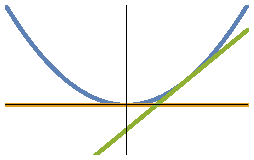
\includegraphics[width=\linewidth]{figures/parabola-linearizations.pdf}}
\noindent\hyperref[fig:parabola-linearizations]{右图}画出了这两个线性化, 与我们从微积分得到的直观认识一致.
\end{Example}

\begin{Example}{球面的线性化}\leavevmode\label{ex:linearizations-of-sphere}
考虑球面 $Y=\mathcal{V}(x^{2}+y^{2}+z^{2}-1)\subseteq\mathbb{A}^{3}_{\mathbb{C}}$, 其 $\mathcal{I}(Y)$ 由 $g=x^{2}+y^{2}+z^{2}-1$ 生成. 为计算在 $a=(0,0,-1)\in Y$ 处的线性化, 先计算生成元的线性化:
\[
  L_{a}g=0(x-0)+0(y-0)+(-2)(z+1)=-2(z+1).
\]
可见 $L_{a}Y=\mathcal{V}(-2(z+1))=\mathcal{V}(z+1)$, 它是包含 $a$ 且平行于 $xy$ 平面的平面.

\BookPairedFigure
  {另一方面, 若考虑点 $b=(1/\sqrt{3},1/\sqrt{3},1/\sqrt{3})\in Y$, 则生成元的线性化为
  \[
    L_{b}g=\frac{2}{\sqrt{3}}\bigl(x+y+z-\sqrt{3}\bigr).
  \]
  因此
  \[
    L_{b}Y=\mathcal{V}\bigl(x+y+z-\sqrt{3}\bigr).
  \]}
  {\phantomsection\label{fig:sphere-linearizations}%
   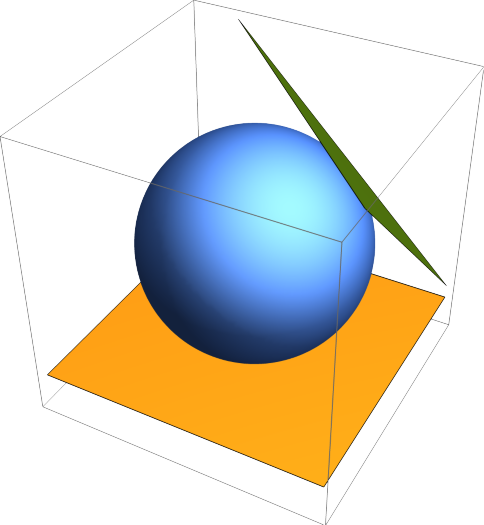
\includegraphics[width=\linewidth]{figures/sphere-linearizations.png}}
\noindent\hyperref[fig:sphere-linearizations]{图中}画出了实数域上的这些线性化, 它们同样符合微积分给出的直观认识.
\end{Example}

\begin{Example}{尖点曲线的线性化}\leavevmode\label{ex:linearizations-of-cusp}
\BookPairedFigure
  {考虑簇 $X=\mathcal{V}(x^{2}-y^{3})\subseteq\mathbb{A}^{2}$, \hyperref[fig:cusp-linearization]{右图}画出它在 $\mathbb{R}$ 上的图形. 如图可见, 这条曲线在原点处有一个\textquotedbl{}尖点\textquotedbl{}, 而在其他各点看上去都\textquotedbl{}光滑\textquotedbl{}. 这一几何观察反映在线性化上.}
  {\phantomsection\label{fig:cusp-linearization}%
   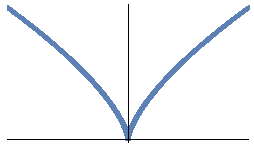
\includegraphics[width=\linewidth]{figures/cusp-linearization.pdf}}
建议读者在 Exercise~\ref{ex:linearizations-of-cusp-at-origin-and-elsewhere} 中验证: $X$ 在原点处的线性化是二维的 (整个 $\mathbb{A}^{2}$), 而在其余任一点处的线性化都是一维的. 在第~\ref{sec:smooth-and-singular-points}~节将看到, 线性化的维数可以用来识别簇中的\textquotedbl{}奇异\textquotedbl{}点, 例如 $X$ 的尖点.
\end{Example}

现在用线性化的概念来定义切空间.

\begin{Definition}{一点处的切向量和切空间}\leavevmode\label{def:tangent-vector-and-tangent-space}
设 $X\subseteq\mathbb{A}^{n}$ 为仿射簇, 且 $a=(a_{1},\ldots,a_{n})\in X$. 对任意 $b=(b_{1},\ldots,b_{n})\in L_{a}X$, 与 $b$ 对应的\emph{切向量}定义为
\[
  \overrightarrow{ab}=(b_{1}-a_{1},\ldots,b_{n}-a_{n})\in K^{n}.
\]
$X$ 在 $a$ 处的\emph{切空间}是所有切向量的集合:
\[
  T_{a}X=\{\overrightarrow{ab}\mid b\in L_{a}X\}\subseteq K^{n}.
\]
\end{Definition}

\BookPairedFigure
  {通常在几何上把切向量 $\overrightarrow{ab}$ 看成在线性化 $L_{a}X$ 内从 $a$ 指向 $b$ 的箭头. 回到 Example~\ref{ex:linearizations-of-sphere} 的单位球面, 取 $a=(0,0,-1)$, 就可以画出一些切向量, 如\hyperref[fig:sphere-tangent-vectors]{右图}所示.

  读到这里, 读者或许 (有理由) 分不清 $L_{a}X$ 和 $T_{a}X$, 这两个对象很相似. 事实上, 自然映射
  \[
    \begin{aligned}
      L_{a}X&\to T_{a}X,\\
      b&\mapsto\overrightarrow{ab}
    \end{aligned}
  \]
  是一个双射, 将 $L_{a}X$ 和 $T_{a}X$ 作为集合认同.}
  {\phantomsection\label{fig:sphere-tangent-vectors}%
   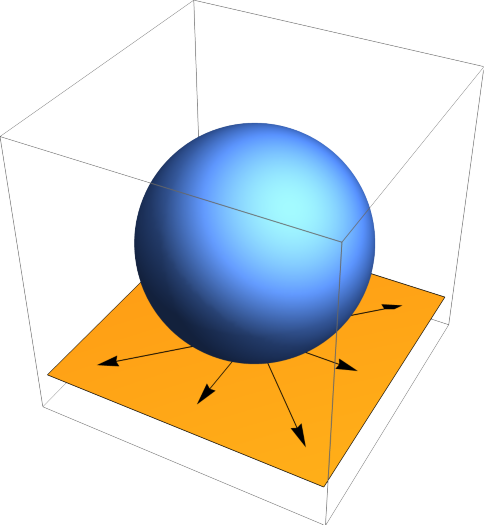
\includegraphics[width=\linewidth]{figures/sphere-tangent-vectors.png}}
那么, 为什么要给这两个相似的对象不同的名称和记号? 原因是我们把 $L_{a}X$ 看成几何对象, 即由 $\mathbb{A}^{n}$ 中的点组成的仿射簇; 而把 $T_{a}X$ 看成代数对象, 由 $K^{n}$ 中的向量组成. 事实上, 如下所见, 集合 $T_{a}X$ 是 $K^{n}$ 的向量子空间. 有了这一关键事实, 就能使用线性代数中的标准工具研究切空间.

在讨论为何切空间是 $K^{n}$ 的向量子空间之前, 先用梯度向量对 $T_{a}X$ 作一个有用的重新解释.

\begin{Definition}{梯度向量}\leavevmode\label{def:gradient-vector}
对任意 $a\in\mathbb{A}^{n}$ 和 $f\in K[x_{1},\ldots,x_{n}]$, $f$ 在 $a$ 处的\emph{梯度}是向量
\[
  \nabla f(a)=\left(\frac{\partial f}{\partial x_{1}}(a),\ldots,
    \frac{\partial f}{\partial x_{n}}(a)\right)\in K^{n}.
\]
\end{Definition}

下面的结论用梯度向量刻画切空间, 这与多元微积分中通常计算切平面的方式类似.

\begin{Proposition}{切空间的梯度刻画}\leavevmode\label{prop:gradient-characterization-of-tangent-spaces}
设 $X\subseteq\mathbb{A}^{n}$ 为仿射簇, 且 $a\in X$. 则
\[
  T_{a}X=\{v\in K^{n}\mid\nabla f(a)\cdot v=0\text{ 对所有 }f\in\mathcal{I}(X)\}.
\]
\end{Proposition}
\begin{Proof}
\BookPairedNoteLeft
  {设 $v=(v_{1},\ldots,v_{n})\in K^{n}$. 由 $T_{a}X$ 的定义可知, $v\in T_{a}X$ 当且仅当对某个 $b\in L_{a}X$, 有 $v=\overrightarrow{ab}$. 展开这个条件, 可知它等价于 $b=(v_{1}+a_{1},\ldots,v_{n}+a_{n})\in L_{a}X$.}
  {Proposition~\ref{prop:gradient-characterization-of-tangent-spaces} 中的\textquotedbl{}$\cdot$\textquotedbl{}是标准点积.}
由 $L_{a}X$ 的定义, $b\in L_{a}X$ 当且仅当对所有 $f\in\mathcal{I}(X)$ 都有
\[
  0=L_{a}f(b)=\sum_{i=1}^{n}\left[\frac{\partial f}{\partial x_{i}}(a)\right](b_{i}-a_{i})
    =\nabla f(a)\cdot v.
\]
因此 $v\in T_{a}X$ 当且仅当对所有 $f\in\mathcal{I}(X)$ 都有 $\nabla f(a)\cdot v=0$.
\end{Proof}

与 $L_{a}X$ 的情形一样, 建议读者验证: 若有一组有限生成元 $\mathcal{I}(X)=\langle f_{1},\ldots,f_{m}\rangle$, 则 Proposition~\ref{prop:gradient-characterization-of-tangent-spaces} 中的消失条件只须在生成元上检查:
\[
  T_{a}X=\{v\in K^{n}\mid\nabla f_{i}(a)\cdot v=0\text{ 对所有 }i=1,\ldots,m\}.
\]
作为 Proposition~\ref{prop:gradient-characterization-of-tangent-spaces} 的推论, 现在证明 $T_{a}X$ 是向量空间.

\begin{Corollary}{切空间是向量空间}\leavevmode\label{cor:tangent-space-is-vector-space}
设 $X\subseteq\mathbb{A}^{n}$ 为仿射簇, 且 $a\in X$. 切空间 $T_{a}X$ 是 $K^{n}$ 的一个向量子空间.
\end{Corollary}
\begin{Proof}
首先, $0\in T_{a}X$, 所以要验证 $T_{a}X$ 是子空间, 只需检查它对这些运算封闭. 设 $v,w\in T_{a}X$ 且 $r\in K$, 须验证 $v-rw\in T_{a}X$. 对任意 $f\in\mathcal{I}(X)$, 有
\[
  \nabla f(a)\cdot(v-rw)=\nabla f(a)\cdot v-r\nabla f(a)\cdot w=0,
\]
其中第一个等号来自点积的线性性, 第二个等号来自 Proposition~\ref{prop:gradient-characterization-of-tangent-spaces} 及假设 $v,w\in T_{a}X$. 因此由 Proposition~\ref{prop:gradient-characterization-of-tangent-spaces} 可知 $v+rw\in T_{a}X$, 证明完毕.
\end{Proof}

从仿射簇 $X\subseteq\mathbb{A}^{n}$ 及点 $a\in X$ 出发, 我们已经定义了向量空间 $T_{a}X\subseteq K^{n}$. 然而, 上面给出的 $T_{a}X$ 的定义是外在的: 它很大程度上依赖于包含关系 $X\subseteq\mathbb{A}^{n}$. 在第~\ref{sec:intrinsic-tangent-spaces}~节, 我们的主要目标是给出 $T_{a}X$ 的内在刻画, 它只依赖于 $K$-代数 $K[X]$ 和极大理想 $I_{a}\subseteq K[X]$, 后者由 $X$ 上在 $a$ 处为零的多项式函数组成. 这个刻画要用到线性代数中的对偶向量空间概念. 因此, 下一节须先稍作迂回, 讨论向量空间的对偶.

\BookExerciseHeading
\begin{BookExercises}
  \item\label{ex:linearization-and-tangency-from-generators} 设 $X\subseteq\mathbb{A}^{n}$ 为仿射簇, $a\in X$, 且 $\mathcal{I}(X)=\langle f_{1},\ldots,f_{m}\rangle$.
  \begin{enumerate}
    \item 证明
    \[
      L_{a}X=\mathcal{V}(L_{a}f_{1},\ldots,L_{a}f_{m}).
    \]
    \item 证明
    \[
      T_{a}X=\{v\in K^{n}\mid\nabla f_{i}(a)\cdot v=0\text{ 对所有 }i=1,\ldots,m\}.
    \]
  \end{enumerate}
  \item\label{ex:defining-polynomial-insufficient-for-linearization} 举出一个仿射簇 $X=\mathcal{V}(f)\subseteq\mathbb{A}^{n}$ 的例子, 使得
  \[
    L_{a}X\neq\mathcal{V}(L_{a}f).
  \]
  换句话说, 计算线性化时仅用定义多项式不够, 而需要用消没理想的生成元.
  \item\label{ex:linearizations-of-cusp-at-origin-and-elsewhere} 设 $X=\mathcal{V}(x^{2}-y^{3})\subseteq\mathbb{A}^{2}$. 证明原点 $(0,0)$ 处的线性化是二维的, 而在其余任一点处的线性化都是一维的.
  \item\label{ex:compare-linearizations-of-paraboloid} 设 $X=\mathcal{V}(x^{2}+y^{2}-z)\subseteq\mathbb{A}^{3}$.
  \begin{enumerate}
    \item 画出 $X$ 在 $\mathbb{R}$ 上的图形.
    \item 证明在 $(0,0,0)$ 处的线性化是三维的, 而在 $X$ 的其余任一点处的线性化都是二维的.
  \end{enumerate}
  \item\label{ex:tangent-space-and-linearization-have-equal-dimension} 对任意仿射簇 $X\subseteq\mathbb{A}^{n}$ 及 $a\in X$, 证明
  \[
    \dim(T_{a}X)=\dim(L_{a}X),
  \]
  其中左边是作为向量空间的维数, 右边是作为仿射簇的维数.
\end{BookExercises}

\par\medskip
{\footnotesize
\noindent\textbf{开放获取.} 本章按照
\href{http://creativecommons.org/licenses/by-nc/4.0/}{Creative Commons Attribution-NonCommercial 4.0 International License}
的条款授权. 该许可允许以任何媒介或格式进行非商业性使用, 分享, 改编, 分发和复制, 但须对原作者和来源作适当署名, 提供 Creative Commons 许可的链接, 并说明是否作了修改.

\noindent
\begin{minipage}[t]{.17\linewidth}
  \vspace{0pt}
\includegraphics[width=.9\linewidth]{figures/source-cc-by-nc.png}
\end{minipage}\hfill
\begin{minipage}[t]{.81\linewidth}
  \vspace{0pt}本章的图片或其他第三方材料均纳入本章的 Creative Commons 许可, 除非材料的署名行另有注明. 如果材料未纳入本章的 Creative Commons 许可, 且您拟进行的使用未获法律规定的许可或超出允许使用的范围, 则须直接向著作权持有人取得许可.
\end{minipage}\par}
